\subsection{}

Advantages of the flyback/Disadvantages of the forward
\begin{itemize}
    \item The forward has a maximum duty $D_{max}$ which is less than 1. This reduces it's operating range.
    \item The flyback has no tertiary winding, which saves on cost.
    \item The flyback uses the coupled coils for energy storage, so there is no additional inductance. Fewer components is cheaper.
    \item The flyback has one less diode. Fewer components is cheaper.
    \item The flyback can both buck and boost. This makes it more versitile.
    \item The forward converter feeds some energy back into the supply each period, which is bad for some supplies.
\end{itemize}

Advantages of the forward/Disadvantages of the flyback
\begin{itemize}
    \item The forward has less ripple than the flyback\todo{does it?}
    \item Since the coupled coils are used for energy storage in the flyback and not in the forward, the core in the forward is physically smaller. This saves on cost.
\end{itemize}

\subsubsection*{Flyback}

\begin{center}
\includegraphics[page=5, 
                     clip, 
                     trim=4cm 9.5cm 3cm 11cm, 
                     width=0.8\textwidth]
                     {5/figures/flyback.pdf} 
\end{center}

\subsubsection*{Forward}

\begin{center}
\includegraphics[page=4, clip, trim=4cm 15cm 2.5cm 7.5cm, scale=0.7]{5/figures/forward.pdf}
\end{center}

